\section{Desarrollo}

  \subsection{Conceptos teóricos}


  % \begin{figure}[h]
  %   \centering
  %   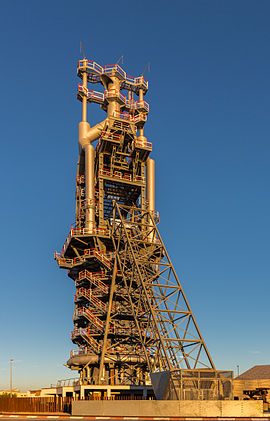
\includegraphics[width=4cm]{altoHorno.jpg}
  %   \caption{Sección horizontal del horno.} \label{fig:seccion-horno}
  % \end{figure}






  \subsection{Aplicación y métodos utilizados}

    \subsubsection{Modelado y planteo del sistema}

 

    \subsubsection{Aplicabilidad de los métodos utilizados}
      


      \begin{prop} \label{prop:La matriz es diagonal dominante}
        La matriz $A \in \mathbb{R}^{(m+1)n \times (m+1)n}$, correspondiente al sistema expuesto en (\ref{des:eq:sistema}), es diagonal dominante, de manera no estricta.
      \end{prop}

      \begin{proof} \ 
        \begin{itemize}
          \item Para las filas $1$ a $n$ de la matriz, correspondientes al borde interno de la discretización, y $mn + 1 $ a $(m+1)n$, correspondientes al borde externo, tenemos que
            \[ A_{p,q} = \begin{cases}
              1 & \text{si $p = q$} \\
              0 & \text{si $p \neq q$}
            \end{cases} \]
          Por lo tanto,
            \[ \vert A_{p,p} \vert = 1 \geq 0 = \sum_{\substack{q=1 \\ q \neq p}}^{(m+1)n} \vert A_{p,q} \vert \]

          \item Las filas $n + 1$ a $mn$ de la matriz corresponden a los puntos $t_{j,k}$ de la discretización con $1 \leq j < m$. En todos estos casos, encontramos solo 5 coeficientes no nulos en la $p$-ésima fila, siendo el que aparece en la diagonal el correspondiente a la variable $t_{j,k}$, y por lo tanto
            \[ \begin{split}
              \vert A_{p,p} \vert &= \left \vert - \frac{2}{(\Delta r)^2} + \frac{1}{r \Delta r} - \frac{2}{r^2 (\Delta \theta)^2} \right \vert \\
              &= \left \vert - \frac{1}{(\Delta r)^2} + \frac{1}{r \Delta r} - \frac{2}{r^2 (\Delta \theta)^2} - \frac{1}{(\Delta r)^2} \right \vert \\
              &= \left \vert - \frac{r - \Delta r}{r (\Delta r)^2} - \frac{2}{r^2 (\Delta \theta)^2} - \frac{1}{(\Delta r)^2} \right \vert \\
              &= \left \vert \frac{r - \Delta r}{r (\Delta r)^2} + \frac{2}{r^2 (\Delta \theta)^2} + \frac{1}{(\Delta r)^2} \right \vert
            \end{split} \]

          Teniendo en cuenta que
            \[ r - \Delta r = (r_i + j \Delta r) - \Delta r = r_i + (j - 1) \Delta r > 0\]
          dado que $r_i, \Delta r > 0$ y $j \geq 1$, es fácil notar que todos los términos que aparecen dentro del módulo son positivos, y por lo tanto
            \[ \vert A_{p,p} \vert = \frac{r - \Delta r}{r (\Delta r)^2} + \frac{2}{r^2 (\Delta \theta)^2} + \frac{1}{(\Delta r)^2} \]

          Por otro lado
            \[ \begin{split}
              \sum_{\substack{q=1 \\ q \neq p}}^{(m+1)n} \vert A_{p,q} \vert &= \left \vert \frac{1}{(\Delta r)^2} - \frac{1}{r \Delta r} \right \vert + 2 \left \vert \frac{1}{r^2 (\Delta \theta)^2} \right \vert + \left \vert \frac{1}{(\Delta r)^2} \right \vert \\
              &= \left \vert \frac{r - \Delta r}{r (\Delta r)^2} \right \vert + \frac{2}{r^2 (\Delta \theta)^2} + \frac{1}{(\Delta r)^2} \\
              &= \frac{r - \Delta r}{r (\Delta r)^2} + \frac{2}{r^2 (\Delta \theta)^2} + \frac{1}{(\Delta r)^2} = \vert A_{p,p} \vert
            \end{split} \]
        \end{itemize}

        De lo anterior, se sigue que
          \[ \vert A_{p,p} \vert \geq \sum_{\substack{q=1 \\ q \neq p}}^{(m+1)n} \vert A_{p,q} \vert \qquad \text{para todo $p = 1, \dots, (m+1)n$} \]
        es decir, $A$ es diagonal dominante de forma no estricta.
      \end{proof}

      \begin{obs}
        \label{obs:Diagonal de A sin ceros}
        Para todo $p = 1, \dots, (m+1)n$, $\vert A_{p,p} \vert > 0$, i.e. la diagonal de $A$ no contiene ceros.
      \end{obs}

      A continuación, probaremos un resultado que nos será útil: al realizar el primer paso de Eliminación Gaussiana sobre una matriz diagonal dominante, la matriz resultante también lo es.



      Nos gustaría demostrar que tanto el método de Eliminación Gaussiana (sin pivoteo) como el de Factorización LU son aplicables en el sistema estudiado. Sin embargo, gracias al siguiente resultado, sabemos que basta con probar que podemos aplicar el primero de ellos, lo cual mostraremos inmediatamente después.



      \begin{prop} \label{prop:Puede aplicarse EG}
        Sea $Ax=b$ la representación matricial correspondiente al sistema expuesto en (\ref{des:eq:sistema}), con $A \in \mathbb{R}^{(m+1)n \times (m+1)n}$ y $b \in \mathbb{R}^{(m+1)n}$ construidos de la manera arriba explicada. Entonces, el sistema $Ax=b$ puede ser resuelto aplicando Eliminación Gaussiana sin pivoteo.
      \end{prop}

      \begin{proof}
        Probaremos que para $u \leq (m+1)n$, es posible realizar $u$ iteraciones de Eliminación Gaussiana sobre $A$ sin pivoteo, y que luego de las mismas, la matriz $A^{(u)}$ resultante es diagonal dominante, con su fila $u + 1$ no nula. Lo haremos por inducción en $u$.

          \begin{itemize}
            \item[\textbf{C.B.}] Teniendo en cuenta que la primera fila de la matriz $A$ tiene necesariamente un $1$ en la diagonal y $0$ en las demás posiciones, se deduce trivialmente que es posible aplicar el primer paso de Eliminación Gaussiana sin realizar pivoteo, dado que $A_{1, 1}$ es no nulo. Del Lema \ref{lema:EG conserva diagonal dominante}, se sigue que la matriz $A^{(1)}$ obtenida será diagonal dominante. Como $A_{1, 2} = 0$, tendremos $A^{(1)}_{2,2} = A_{2,2}$, que es necesariamente no nulo (Observación \ref{obs:Diagonal de A sin ceros}), por lo que la segunda fila de $A^{(1)}$ será no nula.
                
            \item[\textbf{P.I.}] Supongamos que la matriz $A^{(u - 1)}$, obtenida tras aplicar $u - 1$ pasos de Eliminación Gaussiana sobre $A$, es diagonal dominante, con su $u$-ésima fila no nula. Esto implica que $A^{(u - 1)}_{u,u} \neq 0$. Notemos que podemos escribir a $A^{(u - 1)}$ por bloques de la siguiente manera
              \[ A^{(u - 1)} = \left( \begin{matrix} U_{u - 1} & B \\ 0 & \widetilde{A}_{u - 1} \end{matrix} \right) \]
            donde las matrices $U_{u - 1} \in \mathbb{R}^{(u-1)\times(u-1)}$ y $\widetilde{A}_{u - 1} \in \mathbb{R}^{(n-u+1)\times(n-u+1)}$ son trivialmente diagonal dominantes.

            Podemos ver que realizar el paso $u$-ésimo del algoritmo de Eliminación Gaussiana sobre $A$ equivale a realizar el primer paso de este algoritmo sobre $\widetilde{A}_{u - 1}$, sin modificar el resto de la matriz. Dado que $A^{(u - 1)}_{u,u} \neq 0$, podremos realizar esto sin pivoteo, y del Lema 1 se sigue que el resultado de este proceso será diagonal dominante, lo cual implica directamente que también lo será $A^{(u)}$.

            Por último, probemos que la fila $u + 1$ de la matriz $A^{(u)}$ es no nula.
            \begin{itemize}
              \item Si $1 \leq u + 1 \leq n$ o $mn < u + 1 \leq (m+1)n$, tendremos que la fila $u + 1$ tendrá un $1$ en la diagonal y $0$ en las demás posiciones, por lo que no se verá afectada por el algoritmo de Eliminación Gaussiana. Luego $A^{(u)}_{u+1,u+1} = 1$.
              \item En caso contrario, por la forma en la que se construye la matriz del sistema, $A_{u+1,u+1+n}$ corresponde al coeficiente de la variable $t_{j,k+1}$ de la $u + 1$-ésima ecuación del sistema, que es trivialmente no nulo. Además, como notamos anteriormente, la matriz $A$ es \emph{banda} $n, n$. Por lo tanto, $A_{p,u+1+n} = 0$ para todo $p = 0, \dots, u$ y, por consiguiente, $A^{(u)}_{u+1,u+1+n} = A_{u+1,u+1+n}$. Esto implica que la fila $u + 1$ de la matriz $A^{(u)}$ es no nula, como queríamos probar. \qedhere
            \end{itemize}
          \end{itemize}
        \end{proof}

    \subsection{Implementación}

      \subsubsection*{Sustitución hacia adelante y sustitución hacia atrás}
        Como ya mencionamos anteriormente, los dos métodos a utilizar se basan en el hecho de que resolver un sistema de ecuaciones cuya matriz se encuentra en forma triangular (superior o inferior) es sumamente sencillo. Para lograrlo, se utilizan un par de algoritmos sencillos, el de \emph{sustitución hacia adelante} y el de \emph{sustitución hacia atrás}.

        El algoritmo de \emph{sustitución hacia adelante} considera un sistema de ecuaciones $Lx=b$, donde $L$ es una matriz triangular inferior, y devuelve un vector $s$ solución del sistema, con complejidad cuadrática en la cantidad de incógnitas. Lo hace aprovechando el hecho de que el valor de la primera incógnita puede ser despejado de forma inmediata; luego, sustituyendo este valor en la segunda ecuación, puede despejarse la segunda incógnita, y así sucesivamente hasta resolver el sistema completo. El pseudocódigo del algoritmo es el siguiente:

        \vspace*{1em}
        \begin{algorithm}[H]
          \caption{Sustitución hacia adelante}
          \SetKwFunction{sustAdelante}{Sustitución hacia adelante}
          \KwData{$A \in \mathbb{R}^{n \times n}, b \in \mathbb{R}^n$}
          \KwResult{$s \in \mathbb{R}^n$, solución del sistema $Ax=b$, considerando a $A$ como una matriz triangular inferior}
          \For{$i \gets 1$ \KwTo $n$}{
            $suma \gets 0$ \;
            \For{$j \gets 1$ \KwTo $i$}{
              $suma \gets suma + s_j \cdot A_{i,j}$ \;
            }
            $s_i \gets \frac{b_i - suma}{A_{i,i}}$
          }
        \end{algorithm}
        \vspace*{1em}

        El algoritmo de \emph{sustitución hacia atrás} es muy similar al anterior, pero considera un sistema de ecuaciones $Ux=b$, con $U$ triangular superior, y realiza el proceso recorriendo las filas de la matriz en orden inverso, desde abajo hacia arriba.

        \vspace*{1em}
        \begin{algorithm}[H]
          \SetKwFunction{sustAtras}{Sustitución hacia atrás}
          \caption{Sustitución hacia atrás}
          \KwData{$A \in \mathbb{R}^{n \times n}, b \in \mathbb{R}^n$}
          \KwResult{$s \in \mathbb{R}^n$, solución del sistema $Ax=b$, considerando a $A$ como una matriz triangular superior}
          \For{$i \gets n$ \KwTo $1$}{
            $suma \gets 0$ \;
            \For{$j \gets i + 1$ \KwTo $n$}{
              $suma \gets suma + s_j \cdot A_{i,j}$ \;
            }
            $s_i \gets \frac{b_i - suma}{A_{i,i}}$
          }
        \end{algorithm}
        \vspace*{1em}

      \subsubsection*{Eliminación Gaussiana}

        El algoritmo de \emph{Eliminación Gaussiana} permite resolver un sistema de ecuaciones encontrando otro sistema equivalente, pero en forma triangular superior, y luego aplicando el algoritmo de sustitución hacia atrás para hallar la solución del mismo.

        \begin{algorithm}[H]
          \caption{Eliminación Gaussiana}
          \KwData{$A \in \mathbb{R}^{n \times n}, b \in \mathbb{R}^n$}
          \KwResult{$s \in \mathbb{R}^n$, solución del sistema $Ax=b$}
          \For{$j \gets 1$ \KwTo $n$}{
            \For{$i \gets 1$ \KwTo $n$}{
              $m \gets \frac{A_{i,j}}{A_{j,j}}$ \;
              \For{$k \gets j$ \KwTo $n$}{
                $A_{i,k} \gets A_{i,k} - m \cdot A_{j,k}$ \;
              }
              $b_i \gets b_i - m \cdot b_j$ \;
            }
          }
          $s \gets$ \sustAtras{$A,b$} \;
        \end{algorithm}

      \subsubsection*{Factorización LU}

        El algoritmo de \emph{Factorización LU} Permite resolver un sistema de ecuaciones encontrando dos matrices. Una triangular inferior (L) con unos en la diagonal y otra triangular superior (U) que al multiplicarlas dan como resultado la matriz inicial. Luego nos queda $A x = L U x = b$.
        Queremos la solución para un determinando $A$ y $b$. Mediante sustitucion hacia adelante calculamos $y = b * l_{-1}$. Después con sustitucion hacia atras resolvemos  $Ux = y$.

        \begin{algorithm}[H]
          \caption{Factorización LU}
          \KwData{$A \in \mathbb{R}^{n \times n}$}
          \KwResult{$B \in \mathbb{R}^{n \times n}$, tal que los elementos ubicados por encima de y en la diagonal forman una matriz triangular superior $U$, y los ubicados por debajo de la misma, completados con unos en la diagonal, forman una matriz triangular inferior $L$, con $LU=A$}
          \For{$j \gets 1$ \KwTo $n$}{
            \For{$i \gets 1$ \KwTo $n$}{
              $m \gets \frac{A_{i,j}}{A_{j,j}}$ \;
              $B_{i}{j} \gets m$ \;
              \For{$k \gets j+1$ \KwTo $n$}{
                $B_{i,k} \gets A_{i,k} - m \cdot A_{j,k}$ \;
              }
            }
          }
        \end{algorithm}

    \subsubsection{Implementación}

  \subsection{Estimación de la posición de la isoterma y medida de la peligrosidad}

    Una vez obtenida la resolución del sistema, fue necesario decidir un criterio para estimar la ubicación de la isoterma pedida. Algunas de las alternativas que consideramos al respecto fueron las siguientes:

    \begin{itemize}
      \item Para cada ángulo $\theta_k$, considerar como posición de la isoterma el radio correspondiente al punto $(r_j, \theta_k)$ de la discretización con el valor de $t_{j,k}$ más próximo a 500{\degree}C.
      \item Para cada ángulo $\theta_k$, considerar como posición de la isoterma el radio del punto de la discretización inmediatamente exterior al primero con temperatura mayor o igual a 500{\degree}C, contando desde la pared externa. Es decir, considerar el menor radio $r_j$ tal que $t_{j',k} < 500$ para todo $j' \geq j$. La ventaja de este método es que asegura que la isoterma nunca se encontrará más cerca de la pared externa que el resultado arrojado, garantizando que se detectarán todas las posibles situaciones de riesgo.
      \item Para cada ángulo $\theta_k$, considerar $r_j$, el radio del punto más externo de la discretización con temperatura mayor o igual a 500{\degree}C. Luego, sabiendo que la isoterma buscada se encontrará entre este radio y el inmediatamente exterior, aproximar la variación de la temperatura en los puntos intermedios mediante una función lineal y utilizar esta aproximación para estimar la posición de la isoterma. Más precisamente, si $r_{iso}$ es el radio de la isoterma buscada, entonces
        \[ r_{iso} = r_j + \Delta r \left(\frac{500 - t_{j,k}}{t_{j+1,k} - t_{j,k}} \right) \]
    \end{itemize}

    Finalmente, decidimos aplicar este último criterio, porque consideramos que brinda información más precisa que los otros dos, al tener en cuenta el valor la diferencia de temperatura entre los puntos de la discretización más cercanos a la isoterma buscada y la isoterma en si misma, información que los dos primeros métodos descartan. De esta manera, nos permite detectar situaciones de riesgo que con el primer método pasarían desapercibidas, pero evitando la generación de falsos positivos que provocaría el segundo método, que es mucho más estricto.

    Para elegir la medida de peligrosidad lo que hacemos es tomar de todos los valores por los que pasa la isoterma el mas próximo a la pared externa del alto horno. A ese valor lo dividimos por el radio externo, dando así la relación entre la distancia mas cercana a la pared externa de la isoterma y la distancia total.
    Este es un numero entre 1 y 0 donde 0 es el centro del horno y 1 es la pared externa. Cuanto mas cercano a 1 sea el valor, mas peligro de colapsar tiene. 
